\question{考虑矩形谐振腔如图,其中L3>L2>L1. 求\nota{f_{110}}模的磁强。考虑有效电导率,求单位表面的平均损耗功率。}

    \begin{figure}[htbp]
        \centering
        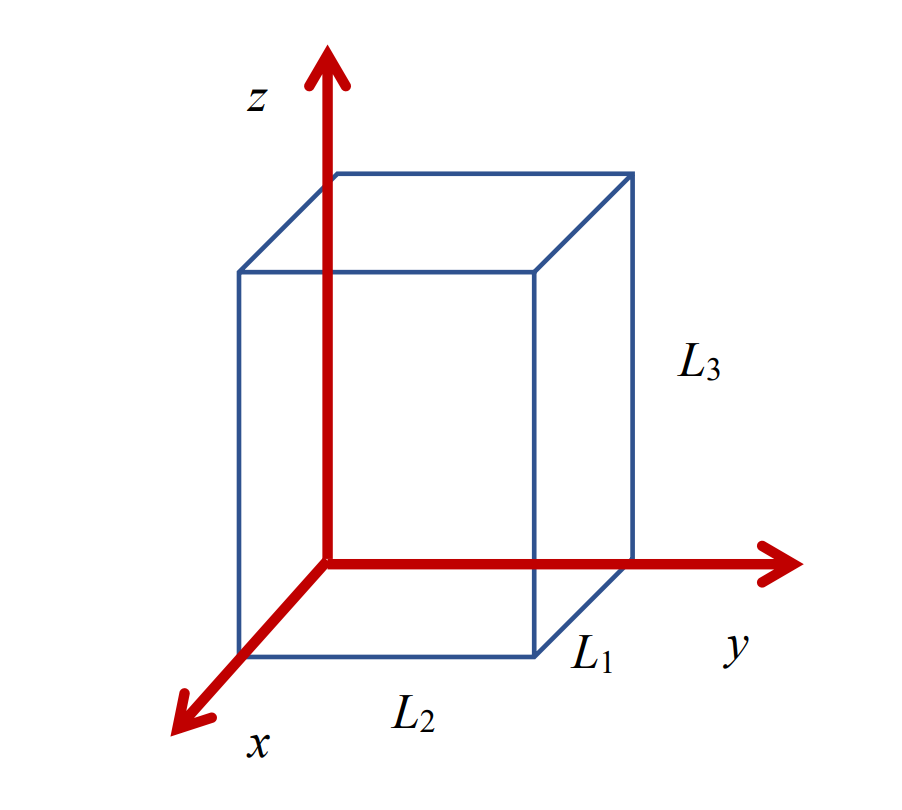
\includegraphics[width=8cm]{img/4.3/1.png}
        \caption{矩形谐振腔}
        \label{4.3_fig:矩形谐振腔}
    \end{figure}
    
    矩形谐振腔中的\nota{f_{110}}模驻波解为
    \equa{\e=E_0\exp{\i\o t}\sin\frac{\pi x}{L_1}\sin\frac{\pi y}{L_2}\bm{e}_z\label{4.3_1}}
    由时谐波的性质得到磁场
    \equa{
        \h=\frac{\exp{\i\o t}}{\i\o\mu}\xuandu\e
        =\frac{\pi E_0\exp{\i\o t}}{\i\o\mu}\kuohao{\frac{1}{L_2}\sin\frac{\pi x}{L_1}\cos\frac{\pi y}{L_2}\bm{e}_x-\frac{1}{L_1}\cos\frac{\pi x}{L_1}\sin\frac{\pi y}{L_2}\bm{e}_y}\label{4.3_2}
    }
    
    由于谐振腔内的驻波解是由理想导体的边界条件得到的,电磁波在导体界面全反射,显然由(\ref{4.3_1})(\ref{4.3_2})可直接算得边界上的平均能流密度为
    \equa{\langle\bm{S}\rangle = \frac{1}{2}\mathrm{Re}\kuohao{\e^*\times\h}=0}
    由于能量守恒,即理想导体边界无损耗功率。
    
    对于非理想导体,考虑良导体条件
    \equa{\xl\ll1}
    我们估计耗散功率密度\nota{p}的一阶小量,即
    \equa{p\sim\O{\xl}\sigma E_0^2}
    对于每个边界,我们从导体内深度为\nota{\xi}处的电流密度入手,计算耗散功率密度,并记\nota{\bm{e}_\xi}为从谐振腔指向导体内部的边界单位法向量。
    
    边界处的切向自由电流线密度矢量\nota{\af}可以由磁场的边界条件确定
    \equa{\af=-\bm{e}_\xi\times\h\label{4.3_af}}
    这里忽略了导体内的磁场,因为它远远小于谐振腔内的磁场\nota{\h}。根据郭硕鸿《电动力学》第四章\nota{\S3}的例2给出的结果,切向\nota{\af}引起的耗散功率体密度\nota{p_t}为
    \equa{p_t\sim\frac{\o\mu}{2}\af^*\cdot\af\exp{-2\alpha\xi}}
    其中
    \equa{\alpha=\sqrt{\frac{\o\mu\sigma}{2}}}
    我们先进行数量级的估算,由(\ref{4.3_2})(\ref{4.3_af})有
    \equa{\af^*\cdot\af\sim\frac{E_0^2}{\o^2\mu^2L^2}}
    于是
    \equa{p_t
        \sim\kuohao{\xl}\sigma\e_0^2\frac{1}{\mu\eps\o^2L^2}
        \sim\kuohao{\xl}\sigma\e_0^2\frac{c^2}{\o^2\lambda^2}\sim\O{\xl}\sigma\e_0^2}
    可见\nota{p_t}为我们要求的一阶小量。
    
    下面估算边界处导体内的法向电流密度的数量级。边界处自由电荷面密度\nota{\sigma_f}满足
    \equa{\sigma_f=-\eps\e\cdot\bm{e}_\xi}
    该式由高斯定律给出,且同样在计算中忽略导体腔内的电场,因为它远远小于谐振腔内电场\nota{\e}(需要注意的是,在计算耗散功率密度时不能忽略导体内电场,因为那个式子两边都是一阶小量)。由电荷的连续性方程可以估算法向电流密度的数量级
    \equa{J_\xi\kuohao{\xi,t}\sim-\pd{\sigma_f}{t}\sim\eps\o E_0}
    则这部分电流的耗散功率密度为
    \equa{p_n=\frac{J_\xi^2}{2\sigma}\sim\O{\kuohao{\xl}^2}\sigma E_0^2} 
    为二阶小量,远远小于切向电流引起的耗散功率密度\nota{p_t}。
    
    于是我们在计算中只需要考虑\nota{p_t}。由(\ref{4.3_2})(\ref{4.3_af})得各个面的耗散功率面密度为
    \equa{
        P_L=
        \left\{
        \begin{aligned}
            &\qquad\qquad\qquad\quad\frac{\pi^2\alpha}{2\sigma\o^2\mu^2}E_0^2\frac{1}{L^2_1}\sin^2\frac{\pi y}{L^2_2} & x=0,L_1 \\
            &\qquad\qquad\qquad\quad\frac{\pi^2\alpha}{2\sigma\o^2\mu^2}E_0^2\frac{1}{L^2_2}\sin^2\frac{\pi x}{L^2_1} & y=0,L_2 \\
            &\frac{\pi^2\alpha}{2\sigma\o^2\mu^2}E_0^2
            \kuohao{
                \frac{1}{L^2_1}\cos^2\frac{\pi x}{L^2_1}\sin^2\frac{\pi y}{L^2_2}+
                \frac{1}{L^2_2}\sin^2\frac{\pi x}{L^2_1}\cos^2\frac{\pi y}{L^2_2}
            }
            & z=0,L_3 \\
        \end{aligned}
        \right.
    }
    % \equa{
    %     P_L=
    %     \begin{cases}
    %         \frac{\pi^2\alpha}{2\sigma\o^2\mu^2}E_0^2\frac{1}{L^2_1}\sin^2\frac{\pi y}{L^2} & x=0,L_1 \\
    %         \frac{\pi^2\alpha}{2\sigma\o^2\mu^2}E_0^2\frac{1}{L^2_1}\sin^2\frac{\pi y}{L^2} & x=0,L_1 \\
    %         \frac{\pi^2\alpha}{2\sigma\o^2\mu^2}E_0^2\frac{1}{L^2_1}\sin^2\frac{\pi y}{L^2} & x=0,L_1 \\
    %     \end{cases}
    % }
    
    % 我们同样可以按照下面的方法考虑有限电导率,再取极限得到这一结果。考虑有限电导率为\nota{\sigma},且有良导体近似\nota{\bm{\alpha}\approx\bm{\beta}\approx(1/\delta)\e'_z},其中定义\nota{\e'_z}为谐振腔指向导体边界方向的法向量,穿透距离为\nota{z'}。在\nota{x=0,L_1}或\nota{y=0,L_2}的边界\nota{\e=0}故亦无电流穿透入导体,而在\nota{z=0,L_3}的边界则有有限的穿透深度。
    % \equa{\e'=E_0\exp{\i\o t}\sin\frac{\pi x}{L_1}\sin\frac{\pi x}{L_2}\exp{\i\kuohao{\beta+\i\alpha}z'}\e'_z}
    % \equa{\bm{J}=\sigma\e'}
    % 单位表面的平均耗散功率为
    % \equa{
    %     \langle P\rangle
    %     =\int_0^\infty\frac{1}{2}\mathrm{Re}\kuohao{\bm{J}^*\times\e'}\d z'
    %     =\frac{\sigma\delta}{4}\kuohao{E_0\sin\frac{\pi x}{L_1}\sin\frac{\pi x}{L_2}}^2
    % }
    % 针对\nota{f_{110}}模进一步化简得到
    % \equa{\langle P\rangle=\frac{1}{4}\sqrt{\frac{2\sigma}{\pi}}\fkuohao{\kuohao{\frac{1}{L_1^2}+\frac{1}{L_2^2}}\frac{\mu}{\eps}}^{-\frac{1}{2}}\kuohao{E_0\sin\frac{\pi x}{L_1}\sin\frac{\pi x}{L_2}}^2}
    % 有趣的是,这一结果显示,电导率\nota{\sigma}趋于无穷时,若不考虑超导效应,耗散功率居然是发散的。
    
\question{论证矩形波导管内不存在\nota{\mathrm{TM}_{m0}}或\nota{\mathrm{TM}_{0n}}波。}

    矩形波导管中的电场单模行波解为
    \begin{equation}
        \left\{
            \begin{aligned}
                    E_x&=A_1\cos(k_xx)\sin(k_yy)\exp{\i k_zz}\\
                    E_y&=A_2\sin(k_xx)\cos(k_yy)\exp{\i k_zz}\\
                    E_z&=A_3\sin(k_xx)\sin(k_yy)\exp{\i k_zz}\\
            \end{aligned}
        \right.
    \end{equation}
    \equa{k_x=\frac{m\pi}{a},\qquad k_y=\frac{n \pi}{b}\qquad(m,n=0,1,2,\cdots)\label{4.3_k}}
    由麦克斯韦方程
    \equa{\h=\frac{1}{\i\o\mu}\xuandu\e}
    得磁场解为
    \begin{equation}
        \left\{
            \begin{aligned}
                    H_x&=(k_yA_3-\i k_zA_2)\sin(k_xx)\cos(k_yy)\exp{\i k_zz}\\
                    H_y&=(\i k_zA_1-k_xA_3)\sin(k_xx)\cos(k_yy)\exp{\i k_zz}\\
                    H_z&=(k_xA_2-k_yA_1)\sin(k_xx)\cos(k_yy)\exp{\i k_zz}\\
            \end{aligned}
        \right.
    \end{equation}
    
    而\nota{\mathrm{TM}}波满足
    \equa{H_z=0}
    对于任意\nota{x,y,z}成立,即
    \nota{k_xA_2-k_yA_1=0\label{4.3_TM}}
    
    则\nota{\mathrm{TM}_{m0}}波要求
    \equa{n=0\label{4.3_n}}
    由(\ref{4.3_k})(\ref{4.3_TM})(\ref{4.3_n})得
    \equa{k_x=k_y=k_z=0}
    即
    \equa{\h_{\mathrm{TM}_{m0}}=0\qquad\e_{\mathrm{TM}_{m0}}=0}
    故矩形波导管内不存在\nota{\mathrm{TM}_{m0}}波。
    
    \nota{\mathrm{TM}_{0n}}波则要求
    \equa{m=0\label{4.3_m}}
    由(\ref{4.3_k})(\ref{4.3_TM})(\ref{4.3_m})得
    \equa{k_x=k_y=k_z=0}
    即
    \equa{\h_{\mathrm{TM}_{0n}}=0\qquad\e_{\mathrm{TM}_{0n}}=0}
    故矩形波导管内不存在\nota{\mathrm{TM}_{0n}}波。
